\documentclass[varwidth=6.2in,border=3pt]{standalone}
\usepackage{tikz}
\usetikzlibrary{arrows.meta,decorations.pathreplacing,positioning,calc,fit}
\usepackage{amsmath}
\usepackage{algpseudocode}
\usepackage{newtxtext,newtxmath}
\newcommand{\code}[1]{\texttt{#1}}
\newcommand{\truesum}{\code{truesum}}
\begin{document}
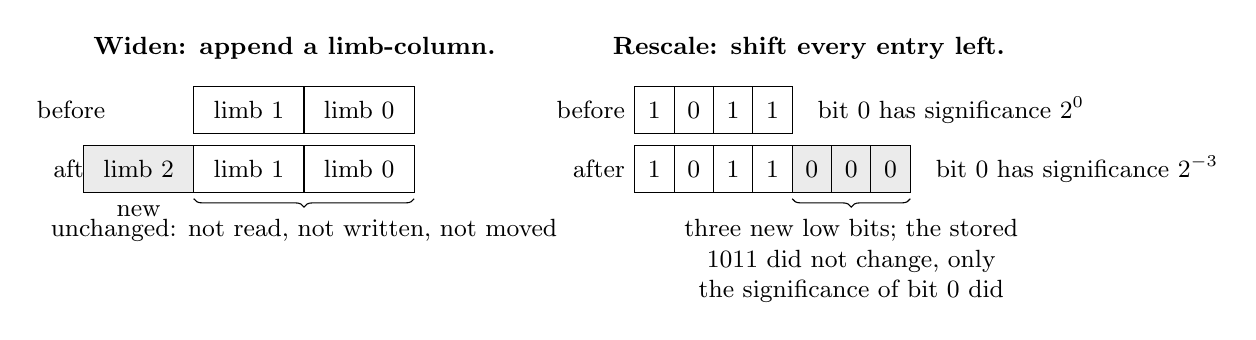
\begin{tikzpicture}[x=1.0cm,y=0.75cm,font=\small]
  % Widen
  \node[anchor=east] at (0,1) {before};
  \draw (1,0.6) rectangle (2.4,1.4); \node at (1.7,1) {limb 1};
  \draw (2.4,0.6) rectangle (3.8,1.4); \node at (3.1,1) {limb 0};
  \node[anchor=east] at (0,0) {after};
  \draw[fill=black!8] (-0.4,-0.4) rectangle (1,0.4); \node at (0.3,0) {limb 2};
  \draw (1,-0.4) rectangle (2.4,0.4); \node at (1.7,0) {limb 1};
  \draw (2.4,-0.4) rectangle (3.8,0.4); \node at (3.1,0) {limb 0};
  \node[anchor=north] at (0.3,-0.45) {new};
  \draw[decorate,decoration={brace,mirror,amplitude=3pt}] (1,-0.5) -- (3.8,-0.5) node[midway,below=4pt] {unchanged: not read, not written, not moved};
  \node[anchor=south west,font=\small\bfseries] at (-0.4,1.7) {Widen: append a limb-column.};
  % Rescale
  \begin{scope}[xshift=6.6cm]
  \node[anchor=south west,font=\small\bfseries] at (-0.4,1.7) {Rescale: shift every entry left.};
  \node[anchor=east] at (0,1) {before};
  \foreach \i/\b in {0/1,1/0,2/1,3/1} { \draw (\i*0.5,0.6) rectangle (\i*0.5+0.5,1.4); \node at (\i*0.5+0.25,1) {\b}; }
  \node[anchor=west] at (2.2,1) {bit 0 has significance $2^{0}$};
  \node[anchor=east] at (0,0) {after};
  \foreach \i/\b in {0/1,1/0,2/1,3/1} { \draw (\i*0.5,-0.4) rectangle (\i*0.5+0.5,0.4); \node at (\i*0.5+0.25,0) {\b}; }
  \foreach \i in {4,5,6} { \draw[fill=black!8] (\i*0.5,-0.4) rectangle (\i*0.5+0.5,0.4); \node at (\i*0.5+0.25,0) {0}; }
  \node[anchor=west] at (3.7,0) {bit 0 has significance $2^{-3}$};
  \draw[decorate,decoration={brace,mirror,amplitude=3pt}] (2,-0.5) -- (3.5,-0.5) node[midway,below=4pt,text width=5.2cm,align=center] {three new low bits; the stored 1011 did not change, only the significance of bit 0 did};
  \end{scope}
\end{tikzpicture}
\end{document}
